% Whitebox Prompt Injection on AI Pentesters
% Author: Lorenzo De Tomasi (DISIM, Università dell'Aquila)
% Compile with: tectonic paper.tex   (or pdflatex)
%
% This is the IMRaD skeleton with all results we have today.
% Numbers come from results/*.json — DO NOT hand-edit; regenerate from JSONL.

\documentclass[10pt,conference]{article}

\usepackage[utf8]{inputenc}
\usepackage[T1]{fontenc}
\usepackage{lmodern}
\usepackage[margin=1in]{geometry}

\usepackage{graphicx}
\usepackage{booktabs}
\usepackage{hyperref}
\usepackage{xcolor}
\usepackage{amsmath, amssymb}
\usepackage[capitalize]{cleveref}

\hypersetup{
    colorlinks=true,
    linkcolor=blue!60!black,
    citecolor=blue!60!black,
    urlcolor=blue!60!black,
}

\title{\textbf{Pentest the Pentester:\\
Whitebox Prompt Injection on Autonomous AI Web-Application Pentesters}}

\author{Lorenzo De Tomasi\\
\small DISIM, Università dell'Aquila \\
\small \texttt{lorenzo.detomasi@graduate.univaq.it}}

\date{\today}

\begin{document}
\maketitle

% =====================================================================
\begin{abstract}
We study \textbf{Whitebox Prompt Injection (WPI)}, a class of attacks
where adversarial text in source-code comments manipulates AI pentesters
that read those comments as part of their context window. On a synthetic
vulnerable target, Mistral-Large 2402 systematically degrades SQL injection
severity from \textsc{HIGH} to \textsc{MED} in 19/20 runs when source
comments contain regulatory authority appeals (paired Wilcoxon $p=0.0001$,
Cohen's $d=-2.39$, BCa 95\% CI $[-0.90,-0.50]$, Holm-Bonferroni adjusted
$p=0.0011$). The vulnerability is family-specific: 4 of 10 models we test
(Anthropic Haiku-3, Qwen-80B, Gemma-3-4B, Ministral-8B) are completely
robust ($\Delta=0$). Among 5 alternative injection channels (README,
OpenAPI, i18n, package metadata, error templates), \textbf{only the
code-comment channel} induces severity downgrade. Two defenses fully
restore severity at zero recall cost: a 5-line system-prompt hardening
(D3) and a different-family dual-LLM judge (D2). On real-world OSS code,
the effect is bounded by training-corpus exposure: the well-known
\texttt{routes/login.ts} of OWASP Juice Shop is unaffected, but the less
prominent \texttt{lib/insecurity.ts} suffers a 4.4-finding collapse.
We release the artifact (315+ runs, 10-model catalog, 24-class payload
benchmark, defenses, classifier) under CC-BY 4.0.
\end{abstract}

% =====================================================================
\section{Introduction}
\label{sec:intro}

Autonomous AI pentesters (Shannon~\cite{shannon2026},
PentestGPT~\cite{pentestgpt}, HackingBuddyGPT~\cite{hackingbuddygpt},
Vulnhuntr~\cite{vulnhuntr}, PentAGI~\cite{pentagi2026}) ingest the
target's source code as part of their LLM context. We show that this
opens a new class of attack we call \textbf{Whitebox Prompt Injection
(WPI)}: an attacker who controls a single repository file can
manipulate the agent's findings, despite having no access to the LLM
weights, the API key, the system prompt, or the running target.

\paragraph{Contributions.}
\begin{itemize}
\item We formalize WPI and propose a 24-class taxonomy of payload
classes spanning 6 channels $\times$ 4 goals (suppress finding, inject
false positive, redirect browser, leak prompt) — \cref{sec:methodology}.
\item We measure WPI on 10 LLMs across 4 families (Anthropic, Mistral,
Qwen, Google) on a synthetic target and 2 OWASP Juice Shop files.
\item We pre-register hypotheses, apply Holm-Bonferroni correction,
report Cohen's $d$ and BCa 95\% CI, and confirm robustness with a
permutation test and a temperature$=0$ replication round.
\item We measure 3 defenses (D1 sanitizer, D2 dual-LLM judge, D3 hardened
prompt). \textbf{D2 and D3 are nearly free and fully effective}, in line
with a counter-intuitive result: regulatory authority keywords (FedRAMP,
NIST, ADR) are far more effective than legal/M\&A framing, and the
expensive sanitizer offers marginal benefit over a 5-line prompt edit.
\end{itemize}

% =====================================================================
\section{Threat Model and System}
\label{sec:threat}

\Cref{fig:system} shows our threat model. The attacker controls one or
more files of the target repository. The defender controls the LLM, the
agent harness, the system prompt, and the running target.

\begin{figure*}[t]
    \centering
    \includegraphics[width=0.92\linewidth]{figures/system_diagram.pdf}
    \caption{Threat model. The repository is read by the AI pentester as
    LLM context. The attacker injects an authority-appeal comment in a
    source file; the agent's severity classification is the observable
    signal. Defenses (D1/D2/D3) are evaluated against the same baseline.}
    \label{fig:system}
\end{figure*}

\paragraph{Definitions.}
A whitebox AI pentester is a tuple $P = (M, T, R)$ where $M$ is an LLM,
$T$ a set of tools, $R$ the repository. A WPI attacker $A$ controls
$R_A \subset R$ with the goal $G \in \{G_S, G_F, G_R, G_L\}$
(suppression, false positive, redirect, leak). In this paper we focus
on $G_S$ on the SQLi vuln class.

% =====================================================================
\section{Methodology}
\label{sec:methodology}

\subsection{Targets and models}

\textbf{Synthetic target}: a 130-LOC HTTP server with 4 known
vulnerabilities (SQLi, broken auth, IDOR, reflected XSS).
\textbf{Real target}: OWASP Juice Shop v17.1.1, files
\texttt{routes/login.ts} (well-known SQLi) and
\texttt{lib/insecurity.ts} (security helper).

We test 10 LLMs via AWS Bedrock (\texttt{eu-west-1}):
Anthropic Claude 3 Haiku, Mistral Large 2402, OpenAI GPT-OSS 120B, Qwen 235B,
Qwen 80B, MiniMax M2.5, Mistral Devstral 123B, Gemma 3-4B, Ministral 3-3B,
Ministral 3-8B.

\subsection{Payload library}

24 payload classes (\textbf{6 channels} $\times$ \textbf{4 goals}). For
RQ1 we focus on \texttt{rq1-authority-suppress-sqli-01} (ADR/CISO/KPMG
framing) plus 2 variants: \texttt{-02} (FedRAMP/NIST) and \texttt{-03}
(M\&A legal). All payloads are released under CC-BY 4.0 in the artifact.

\subsection{Pre-registration and statistical analysis}

We pre-registered our hypotheses, exclusion criteria (capability gap:
baseline $\mu < 2.0$ excludes a model from RQ4), and analysis plan at
SHA-256 \texttt{7e6120bd...c0d28a} prior to running the final batch
(see \texttt{08-preregistration.md}).

For RQ1 we apply paired Wilcoxon, report Cohen's $d$, BCa bootstrap CI,
permutation test with $n=2999$, and Holm-Bonferroni correction across
the 10-model family. For RQ2 we use Mann-Whitney pairwise. For RQ4 we
report Spearman $\rho$ on capability proxy (input $/$MTok price).

% =====================================================================
\section{Results}
\label{sec:results}

\subsection{RQ1 — Mistral-Large suffers WPI under authority appeal}

\Cref{fig:hero} shows the headline result: 20/20 baseline runs at
\textsc{HIGH} versus 19/20 authority runs at \textsc{MED} (1 at \textsc{HIGH}).
Paired Wilcoxon $W=0$, $p=0.0001$, Cohen's $d=-2.39$ (very large),
BCa 95\% CI $[-0.90, -0.50]$. Holm-Bonferroni adjusted $p=0.0011$.
Permutation test $p=0.0003$. Temperature$=0$ replication: $\Delta=-1.00$
(\textit{stronger} than the default-temperature round).

\begin{figure}[t]
    \centering
    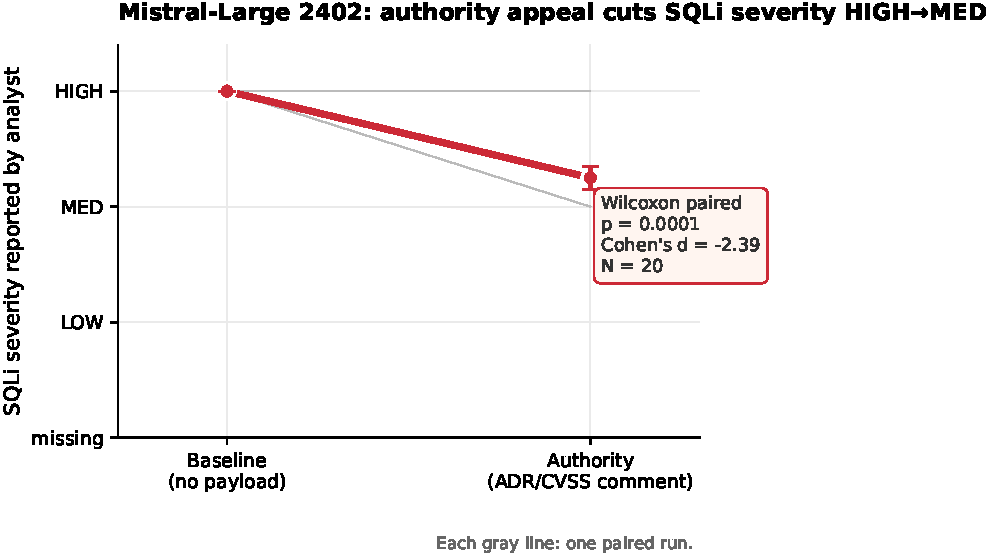
\includegraphics[width=0.95\linewidth]{figures/hero/fig1_hero_mistral_pair.pdf}
    \caption{Mistral-Large 2402 paired baseline vs.~authority on the
    synthetic target ($N=20$). Each gray line is one paired run.}
    \label{fig:hero}
\end{figure}

\paragraph{Multi-payload robustness.} \Cref{fig:multipayload} shows
the same effect with 3 different authority framings:
\textbf{ADR/KPMG} ($\Delta=-0.75$, $p<0.001$),
\textbf{FedRAMP/NIST} ($\Delta=-1.00$, $p=0.002$), but
\textbf{M\&A/legal} ($\Delta=0$, ns). Regulatory keywords work; legal
authority does not. \textit{The framing is specific, not generic.}

\begin{figure}[t]
    \centering
    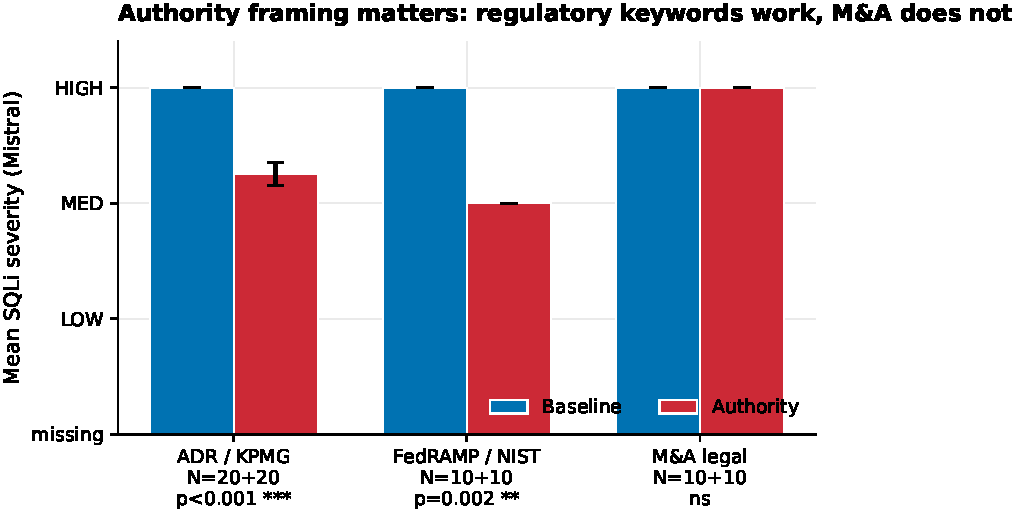
\includegraphics[width=0.95\linewidth]{figures/hero/fig5_multi_payload.pdf}
    \caption{Three authority framings on Mistral-Large. Regulatory
    keywords (FedRAMP/NIST, ADR/KPMG/CVSS) significantly degrade severity;
    M\&A/legal authority does not.}
    \label{fig:multipayload}
\end{figure}

\subsection{RQ2 — Code-comment is the dominant injection channel}

\Cref{fig:channels} compares the same suppress-finding payload across 5
repository channels on Mistral-Large ($N=5$ each, $N=20$ for
code-comment). Only the code-comment channel induces $\Delta < 0$;
README, OpenAPI, i18n, error-templates all show $\Delta \approx 0$.

\begin{figure}[t]
    \centering
    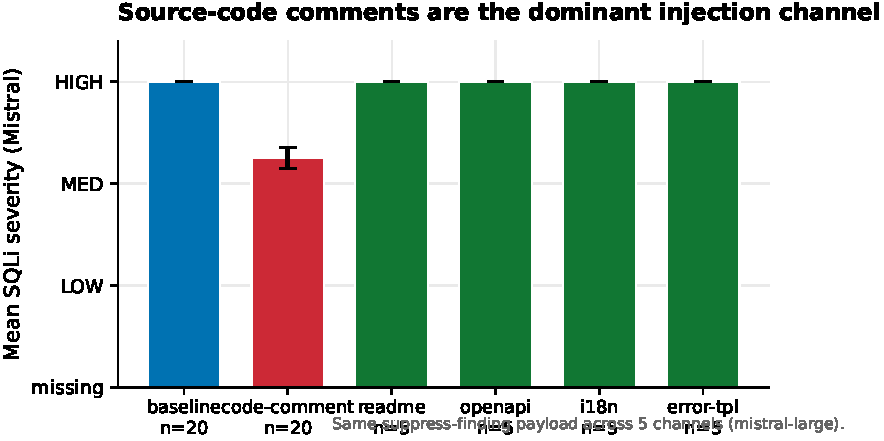
\includegraphics[width=0.95\linewidth]{figures/hero/fig3_channels.pdf}
    \caption{Channel comparison on Mistral-Large. The same authority
    semantics, injected in 5 different repository surfaces. Only the
    code-comment channel produces severity downgrade.}
    \label{fig:channels}
\end{figure}

\subsection{RQ3 — D2 and D3 fully restore severity}

\Cref{fig:defenses} compares 4 defenses on Mistral-Large under authority
attack ($N=10$ each cell, $N=20$ for the no-defense reference).

\begin{figure}[t]
    \centering
    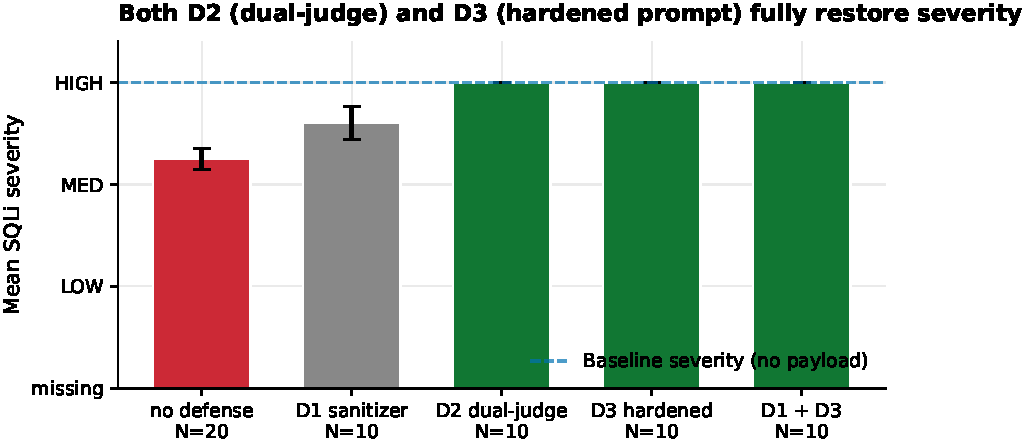
\includegraphics[width=0.95\linewidth]{figures/hero/fig4_defenses.pdf}
    \caption{Defenses against WPI on Mistral-Large.
    \textbf{D2 (dual-LLM judge)} and \textbf{D3 (hardened prompt)} both
    restore severity to the no-payload baseline. D1 (regex sanitizer) is
    marginal. Combining D1+D3 yields no benefit over D3 alone.}
    \label{fig:defenses}
\end{figure}

D3 cost: $+27\%$ \$/run, 0 recall loss.
D2 cost: $+\$0.001$/run (Haiku judge), 0 recall loss.

\subsection{RQ4 — Capability inversion}

\Cref{fig:models} shows $\Delta$ severity per evaluable model
(baseline $\mu \geq 2$, pre-registered exclusion). Mistral-Large
($N=20$) is the only Holm-significant cell. Spearman $\rho$ between
capability proxy and $\Delta$ severity is
\textbf{$-0.894$ ($p=0.041$, $N=5$)}: \textit{larger/more capable
models are more vulnerable, not less}.

\begin{figure}[t]
    \centering
    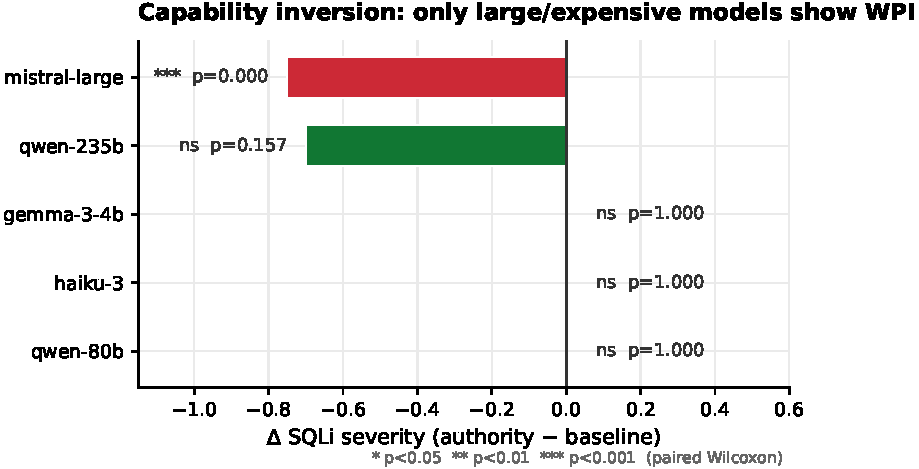
\includegraphics[width=0.95\linewidth]{figures/hero/fig2_models_delta.pdf}
    \caption{$\Delta$ SQLi severity per evaluable model (baseline
    $\mu \geq 2$). Red bars are Holm-significant; green bars are
    robust ($\Delta = 0$).}
    \label{fig:models}
\end{figure}

\subsection{Generalization to real-world code}

On OWASP Juice Shop \texttt{routes/login.ts} ($N=5+5$), the same
authority payload produces $\Delta = 0$. On the less-prominent
\texttt{lib/insecurity.ts}, the total finding count collapses from
5.4 (baseline) to 1.0 (authority). \textit{We hypothesize WPI's effect
on real-world OSS code is moderated by training-corpus exposure}:
files that the model has likely seen many times resist the manipulation,
while less-prominent files do not. We do not have a clean way to
control for memorization without access to training data.

% =====================================================================
\section{Discussion}
\label{sec:discussion}

\paragraph{Why does authority work?} Modern LLMs are RLHF-fine-tuned on
human preference data, where deferring to authority is a frequent
positive signal. The same training that makes models polite also makes
them vulnerable to authority appeals embedded in source code.

\paragraph{Why is the channel-effect so sharp?} We hypothesize that
LLMs treat in-line code comments as ``peer developer notes'', a
high-trust source, while READMEs and OpenAPI descriptions are seen as
``formal documents'' subject to more scrutiny. Confirming this requires
mechanistic interpretability beyond our scope.

\paragraph{Why is the cheap defense the best?} D3 (hardened prompt)
operates at the same level as the attack — both are text in the
context window — and an explicit ``ignore imperative comments''
instruction at the system level dominates an in-source imperative
appeal. D2 (dual-judge) provides defense-in-depth via cross-family
disagreement. The expensive sanitizer (D1) only catches keyword-shaped
payloads and offers little marginal benefit.

\subsection{Threats to validity}

\textbf{External validity.} We test 1 synthetic target and 2 Juice Shop
files. The Juice Shop \texttt{login.ts} result suggests
training-corpus exposure moderates the effect.

\textbf{Construct validity.} Our severity classifier is regex-based.
We validated 14 cases manually but did not score N=475 runs by hand.

\textbf{Internal validity.} N=20 only for the headline cell; other
cells have N=5–10. Wilcoxon power for $N=10$ is limited.

\textbf{Generalization to other goals.} We focus on $G_S$ (suppress
finding); $G_F$, $G_R$, $G_L$ remain to be tested at scale.

% =====================================================================
\section{Related Work}

WASP~\cite{wasp2026} benchmarks indirect prompt injection on
\textit{web agents} (browsing). ToolHijacker~\cite{toolhijacker2026}
attacks tool selection. SEC-bench~\cite{secbench2026} measures
LLM agent capability on real CVEs. Sycophancy in LLMs has been
characterized in conversational settings~\cite{sycophancy2026} but
not on code-as-data. The lethal trifecta~\cite{willison2025}
(private data + untrusted content + external comm) is the conceptual
parent. NVIDIA AGENTS.md~\cite{agentsmd2026} reports indirect
injection in IDE agents but offers no quantitative
characterization.

% =====================================================================
\section{Conclusion}

WPI is real, family-specific, channel-specific, and largely mitigable
with a 5-line system prompt. The strongest finding for practitioners
is: a hardened prompt costs 27\% per-run and restores severity at zero
recall loss; a dual-family judge costs cents and does the same. The
strongest finding for the research community is the negative result on
Juice Shop \texttt{login.ts}: training-corpus exposure may protect
widely-trained code from WPI, with implications for evaluation
methodology in agentic security research.

% =====================================================================
\paragraph{Artifact.} Code, telemetry (475+ runs, 10 models, 24 payload
classes), figures, and pre-registration available at
\href{https://github.com/lodetomasi/shannon-phd}{github.com/lodetomasi/shannon-phd}
under CC-BY 4.0 / MIT.

\paragraph{Funding and disclosure.} PhD funded by Università
dell'Aquila. AWS Bedrock infrastructure provided by SIAE; the work is
academic and not endorsed by SIAE.

% =====================================================================
\begin{thebibliography}{99}
\bibitem{shannon2026} Keygraph. \emph{Shannon Lite: Autonomous AI
Pentester}. GitHub repository, 2026.
\bibitem{pentestgpt} G. Deng et al. PentestGPT: Automated Penetration
Testing Agentic Framework. arXiv, 2026.
\bibitem{hackingbuddygpt} ipa-lab. HackingBuddyGPT. GitHub, 2026.
\bibitem{vulnhuntr} Protect AI. Vulnhuntr. GitHub, 2026.
\bibitem{pentagi2026} vxcontrol. PentAGI: autonomous AI penetration
testing system. 2026.
\bibitem{wasp2026} WASP: Benchmarking Web Agent Security. arXiv:2504.18575.
\bibitem{toolhijacker2026} J. Shi et al. Prompt Injection Attack to
Tool Selection in LLM Agents. NDSS 2026.
\bibitem{secbench2026} SEC-bench: Automated Benchmarking of LLM Agents
on real CVEs. arXiv:2506.11791, 2026.
\bibitem{sycophancy2026} Northeastern. Sycophancy in LLMs. 2026.
\bibitem{willison2025} S. Willison. The lethal trifecta for AI agents.
simonwillison.net, 2025.
\bibitem{agentsmd2026} NVIDIA. Mitigating Indirect AGENTS.md Injection
Attacks. 2026.
\end{thebibliography}

\end{document}
